% Generated by Sphinx.
\def\sphinxdocclass{report}
\documentclass[letterpaper,10pt,english]{sphinxmanual}
\usepackage[utf8]{inputenc}
\DeclareUnicodeCharacter{00A0}{\nobreakspace}
\usepackage{cmap}
\usepackage[T1]{fontenc}
\usepackage{babel}
\usepackage{times}
\usepackage[Bjarne]{fncychap}
\usepackage{longtable}
\usepackage{sphinx}
\usepackage{multirow}


\title{Udrive Documentation}
\date{October 29, 2015}
\release{2}
\author{Grupo5}
\newcommand{\sphinxlogo}{}
\renewcommand{\releasename}{Release}
\makeindex

\makeatletter
\def\PYG@reset{\let\PYG@it=\relax \let\PYG@bf=\relax%
    \let\PYG@ul=\relax \let\PYG@tc=\relax%
    \let\PYG@bc=\relax \let\PYG@ff=\relax}
\def\PYG@tok#1{\csname PYG@tok@#1\endcsname}
\def\PYG@toks#1+{\ifx\relax#1\empty\else%
    \PYG@tok{#1}\expandafter\PYG@toks\fi}
\def\PYG@do#1{\PYG@bc{\PYG@tc{\PYG@ul{%
    \PYG@it{\PYG@bf{\PYG@ff{#1}}}}}}}
\def\PYG#1#2{\PYG@reset\PYG@toks#1+\relax+\PYG@do{#2}}

\expandafter\def\csname PYG@tok@gd\endcsname{\def\PYG@tc##1{\textcolor[rgb]{0.63,0.00,0.00}{##1}}}
\expandafter\def\csname PYG@tok@gu\endcsname{\let\PYG@bf=\textbf\def\PYG@tc##1{\textcolor[rgb]{0.50,0.00,0.50}{##1}}}
\expandafter\def\csname PYG@tok@gt\endcsname{\def\PYG@tc##1{\textcolor[rgb]{0.00,0.27,0.87}{##1}}}
\expandafter\def\csname PYG@tok@gs\endcsname{\let\PYG@bf=\textbf}
\expandafter\def\csname PYG@tok@gr\endcsname{\def\PYG@tc##1{\textcolor[rgb]{1.00,0.00,0.00}{##1}}}
\expandafter\def\csname PYG@tok@cm\endcsname{\let\PYG@it=\textit\def\PYG@tc##1{\textcolor[rgb]{0.25,0.50,0.56}{##1}}}
\expandafter\def\csname PYG@tok@vg\endcsname{\def\PYG@tc##1{\textcolor[rgb]{0.73,0.38,0.84}{##1}}}
\expandafter\def\csname PYG@tok@m\endcsname{\def\PYG@tc##1{\textcolor[rgb]{0.13,0.50,0.31}{##1}}}
\expandafter\def\csname PYG@tok@mh\endcsname{\def\PYG@tc##1{\textcolor[rgb]{0.13,0.50,0.31}{##1}}}
\expandafter\def\csname PYG@tok@cs\endcsname{\def\PYG@tc##1{\textcolor[rgb]{0.25,0.50,0.56}{##1}}\def\PYG@bc##1{\setlength{\fboxsep}{0pt}\colorbox[rgb]{1.00,0.94,0.94}{\strut ##1}}}
\expandafter\def\csname PYG@tok@ge\endcsname{\let\PYG@it=\textit}
\expandafter\def\csname PYG@tok@vc\endcsname{\def\PYG@tc##1{\textcolor[rgb]{0.73,0.38,0.84}{##1}}}
\expandafter\def\csname PYG@tok@il\endcsname{\def\PYG@tc##1{\textcolor[rgb]{0.13,0.50,0.31}{##1}}}
\expandafter\def\csname PYG@tok@go\endcsname{\def\PYG@tc##1{\textcolor[rgb]{0.20,0.20,0.20}{##1}}}
\expandafter\def\csname PYG@tok@cp\endcsname{\def\PYG@tc##1{\textcolor[rgb]{0.00,0.44,0.13}{##1}}}
\expandafter\def\csname PYG@tok@gi\endcsname{\def\PYG@tc##1{\textcolor[rgb]{0.00,0.63,0.00}{##1}}}
\expandafter\def\csname PYG@tok@gh\endcsname{\let\PYG@bf=\textbf\def\PYG@tc##1{\textcolor[rgb]{0.00,0.00,0.50}{##1}}}
\expandafter\def\csname PYG@tok@ni\endcsname{\let\PYG@bf=\textbf\def\PYG@tc##1{\textcolor[rgb]{0.84,0.33,0.22}{##1}}}
\expandafter\def\csname PYG@tok@nl\endcsname{\let\PYG@bf=\textbf\def\PYG@tc##1{\textcolor[rgb]{0.00,0.13,0.44}{##1}}}
\expandafter\def\csname PYG@tok@nn\endcsname{\let\PYG@bf=\textbf\def\PYG@tc##1{\textcolor[rgb]{0.05,0.52,0.71}{##1}}}
\expandafter\def\csname PYG@tok@no\endcsname{\def\PYG@tc##1{\textcolor[rgb]{0.38,0.68,0.84}{##1}}}
\expandafter\def\csname PYG@tok@na\endcsname{\def\PYG@tc##1{\textcolor[rgb]{0.25,0.44,0.63}{##1}}}
\expandafter\def\csname PYG@tok@nb\endcsname{\def\PYG@tc##1{\textcolor[rgb]{0.00,0.44,0.13}{##1}}}
\expandafter\def\csname PYG@tok@nc\endcsname{\let\PYG@bf=\textbf\def\PYG@tc##1{\textcolor[rgb]{0.05,0.52,0.71}{##1}}}
\expandafter\def\csname PYG@tok@nd\endcsname{\let\PYG@bf=\textbf\def\PYG@tc##1{\textcolor[rgb]{0.33,0.33,0.33}{##1}}}
\expandafter\def\csname PYG@tok@ne\endcsname{\def\PYG@tc##1{\textcolor[rgb]{0.00,0.44,0.13}{##1}}}
\expandafter\def\csname PYG@tok@nf\endcsname{\def\PYG@tc##1{\textcolor[rgb]{0.02,0.16,0.49}{##1}}}
\expandafter\def\csname PYG@tok@si\endcsname{\let\PYG@it=\textit\def\PYG@tc##1{\textcolor[rgb]{0.44,0.63,0.82}{##1}}}
\expandafter\def\csname PYG@tok@s2\endcsname{\def\PYG@tc##1{\textcolor[rgb]{0.25,0.44,0.63}{##1}}}
\expandafter\def\csname PYG@tok@vi\endcsname{\def\PYG@tc##1{\textcolor[rgb]{0.73,0.38,0.84}{##1}}}
\expandafter\def\csname PYG@tok@nt\endcsname{\let\PYG@bf=\textbf\def\PYG@tc##1{\textcolor[rgb]{0.02,0.16,0.45}{##1}}}
\expandafter\def\csname PYG@tok@nv\endcsname{\def\PYG@tc##1{\textcolor[rgb]{0.73,0.38,0.84}{##1}}}
\expandafter\def\csname PYG@tok@s1\endcsname{\def\PYG@tc##1{\textcolor[rgb]{0.25,0.44,0.63}{##1}}}
\expandafter\def\csname PYG@tok@gp\endcsname{\let\PYG@bf=\textbf\def\PYG@tc##1{\textcolor[rgb]{0.78,0.36,0.04}{##1}}}
\expandafter\def\csname PYG@tok@sh\endcsname{\def\PYG@tc##1{\textcolor[rgb]{0.25,0.44,0.63}{##1}}}
\expandafter\def\csname PYG@tok@ow\endcsname{\let\PYG@bf=\textbf\def\PYG@tc##1{\textcolor[rgb]{0.00,0.44,0.13}{##1}}}
\expandafter\def\csname PYG@tok@sx\endcsname{\def\PYG@tc##1{\textcolor[rgb]{0.78,0.36,0.04}{##1}}}
\expandafter\def\csname PYG@tok@bp\endcsname{\def\PYG@tc##1{\textcolor[rgb]{0.00,0.44,0.13}{##1}}}
\expandafter\def\csname PYG@tok@c1\endcsname{\let\PYG@it=\textit\def\PYG@tc##1{\textcolor[rgb]{0.25,0.50,0.56}{##1}}}
\expandafter\def\csname PYG@tok@kc\endcsname{\let\PYG@bf=\textbf\def\PYG@tc##1{\textcolor[rgb]{0.00,0.44,0.13}{##1}}}
\expandafter\def\csname PYG@tok@c\endcsname{\let\PYG@it=\textit\def\PYG@tc##1{\textcolor[rgb]{0.25,0.50,0.56}{##1}}}
\expandafter\def\csname PYG@tok@mf\endcsname{\def\PYG@tc##1{\textcolor[rgb]{0.13,0.50,0.31}{##1}}}
\expandafter\def\csname PYG@tok@err\endcsname{\def\PYG@bc##1{\setlength{\fboxsep}{0pt}\fcolorbox[rgb]{1.00,0.00,0.00}{1,1,1}{\strut ##1}}}
\expandafter\def\csname PYG@tok@kd\endcsname{\let\PYG@bf=\textbf\def\PYG@tc##1{\textcolor[rgb]{0.00,0.44,0.13}{##1}}}
\expandafter\def\csname PYG@tok@ss\endcsname{\def\PYG@tc##1{\textcolor[rgb]{0.32,0.47,0.09}{##1}}}
\expandafter\def\csname PYG@tok@sr\endcsname{\def\PYG@tc##1{\textcolor[rgb]{0.14,0.33,0.53}{##1}}}
\expandafter\def\csname PYG@tok@mo\endcsname{\def\PYG@tc##1{\textcolor[rgb]{0.13,0.50,0.31}{##1}}}
\expandafter\def\csname PYG@tok@mi\endcsname{\def\PYG@tc##1{\textcolor[rgb]{0.13,0.50,0.31}{##1}}}
\expandafter\def\csname PYG@tok@kn\endcsname{\let\PYG@bf=\textbf\def\PYG@tc##1{\textcolor[rgb]{0.00,0.44,0.13}{##1}}}
\expandafter\def\csname PYG@tok@o\endcsname{\def\PYG@tc##1{\textcolor[rgb]{0.40,0.40,0.40}{##1}}}
\expandafter\def\csname PYG@tok@kr\endcsname{\let\PYG@bf=\textbf\def\PYG@tc##1{\textcolor[rgb]{0.00,0.44,0.13}{##1}}}
\expandafter\def\csname PYG@tok@s\endcsname{\def\PYG@tc##1{\textcolor[rgb]{0.25,0.44,0.63}{##1}}}
\expandafter\def\csname PYG@tok@kp\endcsname{\def\PYG@tc##1{\textcolor[rgb]{0.00,0.44,0.13}{##1}}}
\expandafter\def\csname PYG@tok@w\endcsname{\def\PYG@tc##1{\textcolor[rgb]{0.73,0.73,0.73}{##1}}}
\expandafter\def\csname PYG@tok@kt\endcsname{\def\PYG@tc##1{\textcolor[rgb]{0.56,0.13,0.00}{##1}}}
\expandafter\def\csname PYG@tok@sc\endcsname{\def\PYG@tc##1{\textcolor[rgb]{0.25,0.44,0.63}{##1}}}
\expandafter\def\csname PYG@tok@sb\endcsname{\def\PYG@tc##1{\textcolor[rgb]{0.25,0.44,0.63}{##1}}}
\expandafter\def\csname PYG@tok@k\endcsname{\let\PYG@bf=\textbf\def\PYG@tc##1{\textcolor[rgb]{0.00,0.44,0.13}{##1}}}
\expandafter\def\csname PYG@tok@se\endcsname{\let\PYG@bf=\textbf\def\PYG@tc##1{\textcolor[rgb]{0.25,0.44,0.63}{##1}}}
\expandafter\def\csname PYG@tok@sd\endcsname{\let\PYG@it=\textit\def\PYG@tc##1{\textcolor[rgb]{0.25,0.44,0.63}{##1}}}

\def\PYGZbs{\char`\\}
\def\PYGZus{\char`\_}
\def\PYGZob{\char`\{}
\def\PYGZcb{\char`\}}
\def\PYGZca{\char`\^}
\def\PYGZam{\char`\&}
\def\PYGZlt{\char`\<}
\def\PYGZgt{\char`\>}
\def\PYGZsh{\char`\#}
\def\PYGZpc{\char`\%}
\def\PYGZdl{\char`\$}
\def\PYGZhy{\char`\-}
\def\PYGZsq{\char`\'}
\def\PYGZdq{\char`\"}
\def\PYGZti{\char`\~}
% for compatibility with earlier versions
\def\PYGZat{@}
\def\PYGZlb{[}
\def\PYGZrb{]}
\makeatother

\begin{document}

\maketitle
\tableofcontents
\phantomsection\label{index::doc}


Contents:


\bigskip\hrule{}\bigskip



\chapter{UDrive - Entrega}
\label{uDriveDoc:welcome-to-udrive-s-documentation}\label{uDriveDoc:udrive-entrega}\label{uDriveDoc::doc}
\textbf{30/10/2015}

\textbf{Grupo Nro 5}

\textbf{Ayudante asignado: Pablo Rodríguez Manzi}

\textbf{Integrantes:}

\begin{tabulary}{\linewidth}{|L|L|}
\hline
\textsf{\relax 
Apellido y Nombre
} & \textsf{\relax 
Padrón
}\\
\hline
Cortazzo Romina Pamela
 & 
80915
\\
\hline
D'Onofrio Martín
 & 
82106
\\
\hline
Liva María Eugenia
 & 
86123
\\
\hline
Quiroz Martín
 & 
86012
\\
\hline\end{tabulary}


\textbf{Tag a descargar:}


\bigskip\hrule{}\bigskip



\chapter{Manual de proyecto}
\label{uDriveDoc:manual-de-proyecto}

\section{Gestión del proyecto}
\label{uDriveDoc:gestion-del-proyecto}
Las tareas se gestionaron mediante el sistema de tickets que nos proveé GitHub. Por cada tarea a realizar se crea un issue que se asigna a un integrante del grupo.
Para tener una trazabilidad del estado de las tareas y el código que corresponde a cada corrección, al realizar un commit se indica el número de issue al que corresponde. Por tal razón al momento de  definir las tareas se tuvo en cuenta que sean lo suficientemente atómicas como para cerrarlas con un único commit.


\section{División de tareas}
\label{uDriveDoc:division-de-tareas}
Para el desarrollo de UDrive se conformaron los módulos Cliente y Servidor, asignando a dos integrantes del equipo a cargo principalmente de uno de los módulos. Lo cual puede cambiar de ser necesario. Las asignaciones fueron:
\begin{itemize}
\item {} 
Cliente:  Liva María Eugenia y Cortazzo Romina Pamela

\item {} 
Servidor:  Quiroz Martín y D'Onofrio Martín

\end{itemize}


\section{Tareas que componen el checklist nro 2}
\label{uDriveDoc:tareas-que-componen-el-checklist-nro-2}
Son todas las pertenecientes al milestone \href{https://github.com/martineq/tp7552/milestones/Checkpoint\%20\%232}{Checkpoint \#2}


\section{Funcionalidad entregada en el checklist nro 2}
\label{uDriveDoc:funcionalidad-entregada-en-el-checklist-nro-2}
En esta entrega se incluye a nivel funcionalidad:

\textbf{Cliente:}
\begin{itemize}
\item {} 
Configuración de la ip del servidor del cual se consumen los servicios (Connection Settings).

\item {} 
Registración de un nuevo usuario (Sign Up).

\item {} 
Carga de un archivo (Add file).

\item {} 
Creación de una carpeta (Add folder).

\item {} 
Administración de perfil de usuario (My profile).

\end{itemize}

\textbf{Servidor:}
\begin{itemize}
\item {} 
Integración con la base de datos del servicio de optención de token y lista de archichos.

\item {} 
Implementación de servicio de creación de carpeta.

\item {} 
Implementación de servicio de carga de archivo.

\item {} 
Implementación de servicio de registración de usuario.

\end{itemize}


\section{Control de versiones - Repositorio}
\label{uDriveDoc:control-de-versiones-repositorio}
El control de versiones del proyecto fue mediante Github.
Se utilizaron un mismo repositorio para el proyecto de servidor y del cliente.

\href{https://github.com/martineq/tp7552.git}{Repositorio}

El manejo de branches que realizamos es el siguiente:
\begin{itemize}
\item {} 
Master: Sólo se hará commit sobre este branch al momento de cerrar un checkpoint.

\item {} 
Develop: Se subirán a este branch las funcionalidades que se vayan cerrando.

\item {} 
Features branches: Cada integrante trabajará en una branch local y una vez que tenga la funcionalidad terminada, hará merge con Develop y volcará sobre este los cambios.

\end{itemize}


\bigskip\hrule{}\bigskip



\chapter{Manual Técnico}
\label{uDriveDoc:manual-tecnico}

\section{API REST}
\label{uDriveDoc:api-rest}
Para la comunicación entre Cliente y Servidor se definieron los siguientes servicios REST:
\begin{itemize}
\item {} 
\textbf{Agrega un archivo en el directorio indicado}

\end{itemize}
\begin{itemize}
\item {} 
URL: /users/\{userId\}/dir/\{dirId\}

\item {} 
Verbo: POST

\item {} \begin{description}
\item[{Ejemplo de entrada (multipart):}] \leavevmode
``file'': binario
``filename'': ``archivo.txt''

\end{description}

\item {} \begin{description}
\item[{Ejemplo de salida (JSON):}] \leavevmode
``id'': 1,
``name'': ``Carpeta1'',
``size'': 1234,
``type'': ``d'',
``cantItems'': 2,
``shared'': true,
``lastModDate'': ``10/08/2015''
\},
\{
``id'': 2
``name'': ``Carpeta2'',
``size'': 500,
``type'': ``a'',
``cantItems'': 1
``shared'': false,
``lastModDate'': ``10/08/2015''
\},
...
{]}

\end{description}

\end{itemize}
\begin{itemize}
\item {} 
\textbf{Crea un directorio en el directorio}

\end{itemize}
\begin{itemize}
\item {} 
URL: /users/\{userId\}/dir/\{dirId\}

\item {} 
Verbo: POST

\item {} \begin{description}
\item[{Ejemplo de entrada (JSON):}] \leavevmode
\{``dirName'': ``nuevo\_directorio''\}

\end{description}

\item {} \begin{description}
\item[{Ejemplo de salida (JSON):}] \leavevmode
``id'': 1,
``name'': ``Carpeta1'',
``size'': 1234,
``type'': ``d'',
``cantItems'': 2,
``shared'': true,
``lastModDate'': ``10/08/2015''
\},
\{
``id'': 2
``name'': ``Carpeta2'',
``size'': 500,
``type'': ``a'',
``cantItems'': 1
``shared'': false,
``lastModDate'': ``10/08/2015''
\},
...
{]}

\end{description}

\end{itemize}
\begin{itemize}
\item {} 
\textbf{Registración de usuario}

\end{itemize}
\begin{itemize}
\item {} 
URL: /signup

\item {} 
Verbo: POST

\item {} 
Descripción: Chequea si el e-mail enviado existe o no. Si existe devuelve un código de error ( != 1).De lo contrario inserta todos los campos recibidos en la base de datos y devuelve un código de operación exitosa (1).

\item {} \begin{description}
\item[{Ejemplo de entrada (JSON):}] \leavevmode\begin{description}
\item[{\{}] \leavevmode
``firstname'': ``nombre'',
``lastname'': ``apellido'',
``email'': ``\href{mailto:mail@mail.com}{mail@mail.com}'',
``password'': ``xxxxxxxx''

\end{description}

\}

\end{description}

\item {} \begin{description}
\item[{Ejemplo de salida (JSON):}] \leavevmode\begin{description}
\item[{\{}] \leavevmode
``resultCode'': 1

\end{description}

\}

\end{description}

\end{itemize}
\begin{itemize}
\item {} 
\textbf{Consulta de perfil de usuario}

\end{itemize}
\begin{itemize}
\item {} 
URL: /profile/\{userId\}

\item {} 
Verbo: GET

\item {} 
Descripción: Trae todos los campos pertenecientes al perfil del usuario logueado en la aplicación.

\item {} \begin{description}
\item[{Ejemplo de salida (JSON):}] \leavevmode\begin{description}
\item[{\{}] \leavevmode
``firstname'': ``nombre'',
``lastname'': ``apellido'',
``email'': ``\href{mailto:mail@mail.com}{mail@mail.com}'',
/\emph{``photo'': ``dfd5g46s5gfGf'',}/
/\emph{``lastLocation'': ``'',}/
``userId'': ``5'',
``quotaAvailable'': ``570 MB''
``quotaTotal'': ``756 MB''
``quotaUsagePercent'': ``75.39\%''

\end{description}

\}

\end{description}

\end{itemize}


\section{Base de Datos}
\label{uDriveDoc:base-de-datos}
Para persistir los datos se utilizó RocksDB

\textbf{Información que se necesitaba persistir}
\begin{itemize}
\item {} 
Relacionados a un cliente (user):

\end{itemize}
\begin{itemize}
\item {} 
user\_id

\item {} 
user\_email

\item {} 
user\_password

\item {} 
user\_token

\item {} 
user\_name

\item {} 
user\_location

\item {} 
user\_dir\_root

\item {} 
user\_shared\_files

\end{itemize}
\begin{itemize}
\item {} 
Relacionados a un directorio (directory):

\end{itemize}
\begin{itemize}
\item {} 
dir\_id

\item {} 
dir\_name

\item {} 
dir\_date\_last\_mod

\item {} 
dir\_tags

\item {} 
dir\_owner

\item {} 
dir\_parent\_directory

\item {} 
dir\_files\_contained

\item {} 
dir\_directories\_contained

\end{itemize}
\begin{itemize}
\item {} 
Relacionados a un archivo (file):

\end{itemize}
\begin{itemize}
\item {} 
file\_id

\item {} 
file\_name

\item {} 
file\_extension

\item {} 
file\_date\_last\_mod

\item {} 
file\_user\_last\_mod

\item {} 
file\_tags

\item {} 
file\_owner

\item {} 
file\_size (expresado en Kilobytes)

\item {} 
file\_deleted\_status

\item {} 
file\_users\_shared

\item {} 
file\_revision

\end{itemize}
\begin{itemize}
\item {} 
Relacionados a la búsquedas por atributos que no son el ID (index):

\end{itemize}
\begin{itemize}
\item {} 
index\_user\_id\_from\_user\_email

\end{itemize}
\begin{itemize}
\item {} 
Relacionados al manejo de asignaciones de id para usuarios, directorios y archivos (ticket):

\end{itemize}
\begin{itemize}
\item {} 
ticket\_last\_user\_id

\item {} 
ticket\_last\_dir\_id

\item {} 
ticket\_last\_file\_id

\end{itemize}


\section{Servidor}
\label{uDriveDoc:servidor}
\textbf{Diagrama de clases}

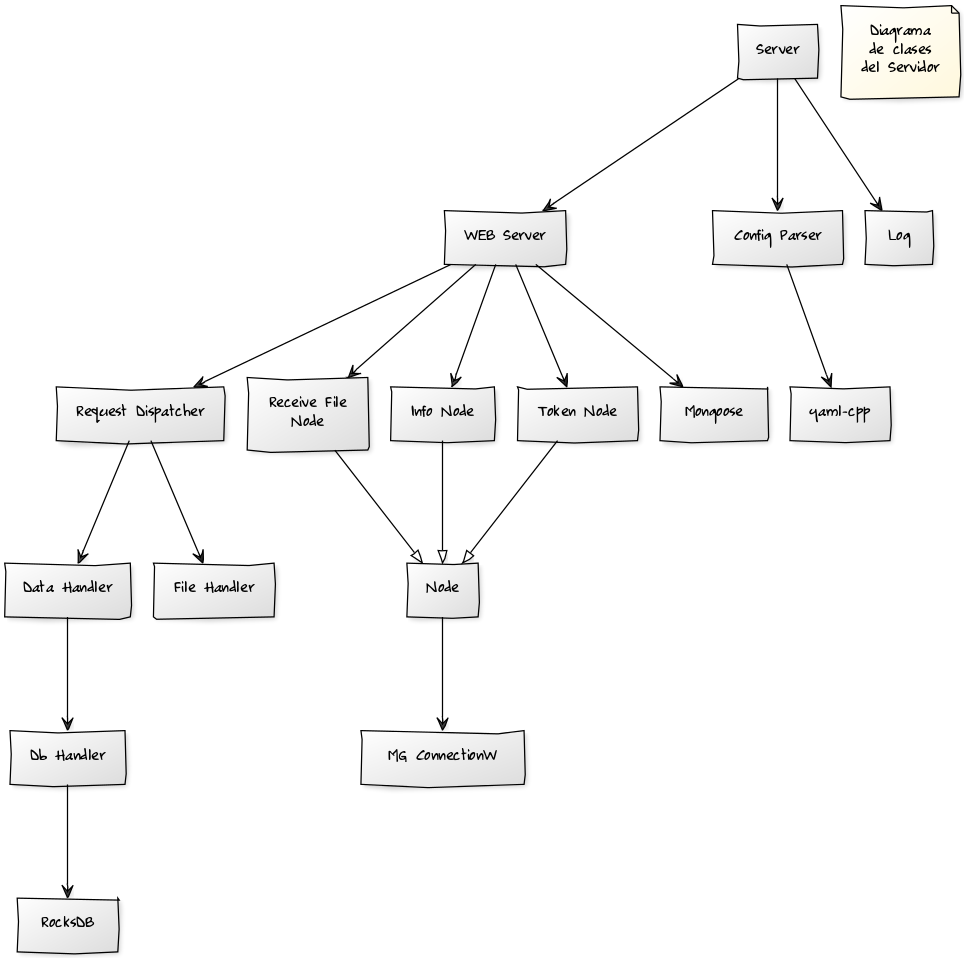
\includegraphics{diagrama_clase_serv.png}

\textbf{Instalacón y configuración}
\begin{enumerate}
\item {} 
Descargar el \href{https://raw.githubusercontent.com/martineq/tp7552/master/server/server\_install\_v0.1.sh}{script de instalación}

\item {} \begin{description}
\item[{Para la instalación:}] \leavevmode\begin{enumerate}
\item {} 
chmod 777 server\_install\_v0.1.sh

\item {} 
./server\_install\_v0.1.sh

\end{enumerate}

\end{description}

\item {} \begin{description}
\item[{Luego ejecutar el servidor con:}] \leavevmode\begin{enumerate}
\item {} 
./server

\end{enumerate}

\end{description}

\end{enumerate}

\textbf{Ejecución de pruebas}

Luego de haber levantado el servidor con los pasos indicados anteriormente, ejecutar:
\begin{itemize}
\item {} 
cmake -DCOVERALLS=ON -DCMAKE\_BUILD\_TYPE=Debug ..

\item {} 
make

\item {} 
make coveralls

\end{itemize}


\section{Cliente}
\label{uDriveDoc:cliente}
\textbf{Instalacón y configuración}
\begin{enumerate}
\item {} 
Descargar el \href{https://github.com/martineq/tp7552/raw/344e1550a2eab0febc324910d4edaf2256522ac9/client/src/Udrive/app/app-release.apk}{apk de instalación}

\item {} 
Configurar ip del servidor entrando a Settings \textgreater{} Connection settings

\end{enumerate}

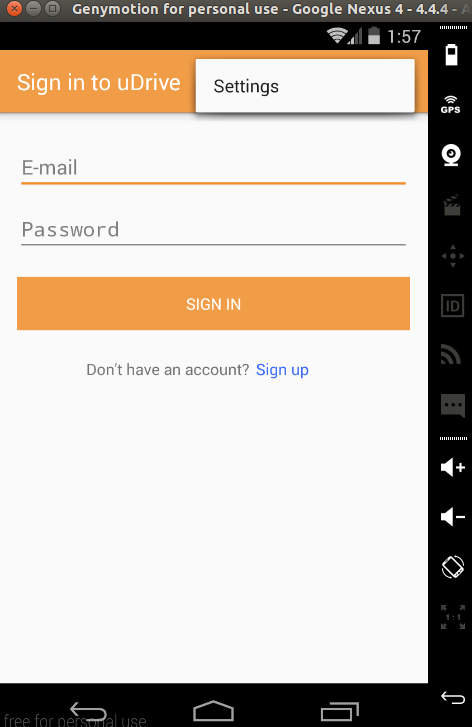
\includegraphics{settings.png}

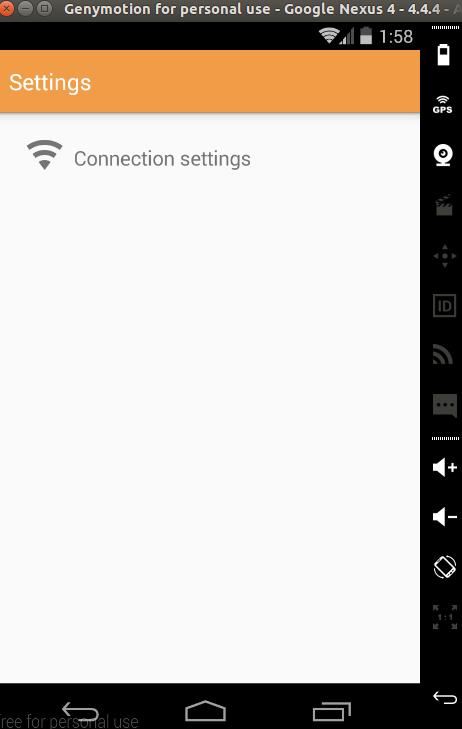
\includegraphics{connectionSettings1.png}

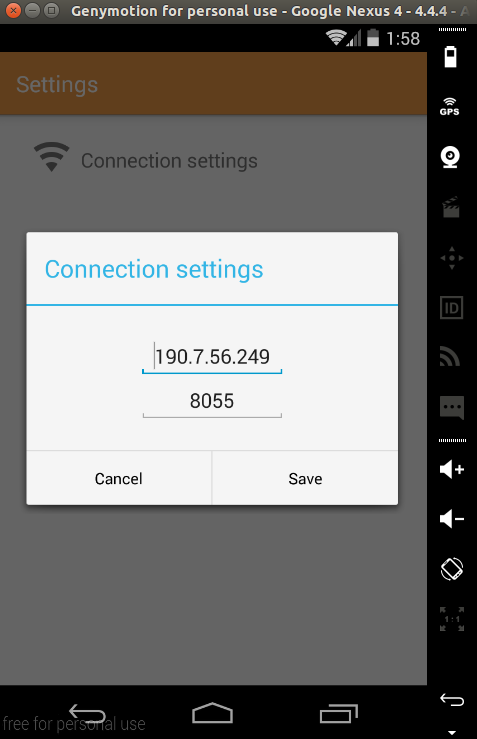
\includegraphics{connectionSettings2.png}


\chapter{Indices and tables}
\label{index:indices-and-tables}\begin{itemize}
\item {} 
\emph{genindex}

\item {} 
\emph{modindex}

\item {} 
\emph{search}

\end{itemize}



\renewcommand{\indexname}{Index}
\printindex
\end{document}
